% !TEX encoding = UTF-8 Unicode
\documentclass[a4paper]{article}

\usepackage[utf8]{inputenc}
\usepackage{erk}
\usepackage{times}
\usepackage{graphicx}
\usepackage[top=22.5mm, bottom=22.5mm, left=22.5mm, right=22.5mm]{geometry}

\usepackage[slovene,english]{babel}

% local definitions
\def\footnotemark{}%  to avoid footnote on cover page

\begin{document}
%make title
\title{WSN(BSO) final report}

\author{Denis Vitez$^{1}$, Luka Golinar$^{1}$} % use ^1, ^2 for author(s) from different institutions

\affiliation{$^{1}$University of Ljubljana, FRI}

\email{E-mail: dv9763@student.uni-lj.si, lgxxxx@student.uni-lj.si}

\maketitle

%\thispagestyle{empty}

\begin{abstract}{Abstract}
This paper will present the finding and results of a final seminar project at subject WSN (Wireless sensor networks).
\end{abstract}


\selectlanguage{english}

\section{Problem}
The problem that we had to tackle in the seminar project was to develop an wireless sensor network, that will use physical Zolertia Z1 motes and also virtual motes inside Cooja program that is bundled with the Contiki operating system, that was running on our devices. The resulting network had to be robust, so it would handle failure of one or multiple motes and also the requirement for the network had to use multihop, since not all nodes were in direct range with one another. After the network has been setup, we had to implemented differenc actions that the network could perform. For example network had to return results for given queries (temperature, vibration level, ...). The other requirement was for the network to be able to detect anomalies and report them to the "master" node.
\section{Design}

\section{Implementation}
\subsection{Routing}
\subsection{Commands}
Commands are issued in SCPI - 99 compliant standard. They are represented with the following structure: \textbf{NETWORK:FAMILY:FUNCTION:PART}.
\begin{figure}[!htb]
    \begin{center}
        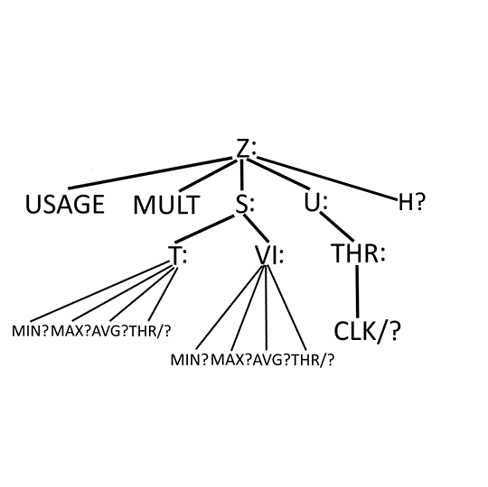
\includegraphics[scale=0.8]{structure.png}
        \caption{Tree structure of messages.} \label{pic1}
    \end{center}
\end{figure}

In out assignment we had to support the following queries (Q) and alarms (A):
\begin{itemize}
\item \textbf{Q:} Maximum temperature across the whole network.
\item \textbf{Q:} Minimum temperature across the whole network.
\item \textbf{Q:} Find nodes with maximum vibration level.
\item \textbf{Q:} Average vibration level across the whole network.
\item \textbf{Q:} Find currently connected nodes (heartbeat).
\item \textbf{A:} Report if temperature at some sensor exceeds a certain threshold.
\item \textbf{A:} Report if vibration at some sensor exceeds a certain threshold.
\end{itemize}
\section{Optimization}
\subsection{Power consumption}
\subsection{Memory usage}
\section{Results}
Results and graphs from Cooja should go here...
\small
\begin{thebibliography}{1}

\bibitem{ERK} ERK, http://www.ieee.si/erk/index.html 
\bibitem{Zbornik} B. Zajc, A. Trost: Zbornik triindvajsete mednarodne Elektrotehniške in računalniške konference ERK 2014, 22. - 24. September 2014, Portorož, Slovenija

\end{thebibliography}

\end{document}
